\chapter{Fejlesztői dokumentáció} % Developer guide
\label{ch:developer}

\section{Keretrendszer és az alkalmazás felépítése}
\label{sec:framework-app}
\subsection{Keretrendszer}
\label{subsec:framework}
Az alkalmazás ASP.NET core 3.1 keretrendszerben készült \cite{ASPDOTNETCORE3_1}, ami egy nyílt forráskódú, webes alkalmazások készítésére szolgáló programkönyvtár, melyet a \emph{Microsoft} fejleszt. A keretrendszer lehetővé teszi, hogy az alkalmazás több platformon is tudjon futni (\emph{Linux}, \emph{macOS} és \emph{Windows}). Továbbá az alkalmazás rendelkezik autentikációval és autorizációval.
\subsection{Az alkalmazás felépítése}
\label{subsec:app} 
Az alkalmazás az \emph{MVC} architektúrára épül (\ref{fig:mvc-pattern} ábra)\cite{MVC}. Tehát három rétegre bontható a felépítése, Modell-Nézet-Vezérlő. A Modell réteg tartalmazza az üzleti logikát, amely az adatokat kezeli és kapcsolatban van az adatbázissal. A nézet réteg (angolul \emph{View}) felelős a megjelenítésért. A vezérlő réteg (angolul \emph{Controller}) fogadja a kliens a kéréseit és válaszol a kérésekre. Az \emph{MVC} architektúra fő előnye, hogy jól elkülöníthetőek a rétegek, így a nézet független marad a modelltől. Ezáltal, ha szükséges könnyedén le tudjuk cserélni az egész alkalmazás nézetét, vagy fordítva újra implementálhatjuk a modell réteg működését, anélkül hogy ez a nézeten bármi gondot okozna.
\begin{figure}[H]
	\centering
	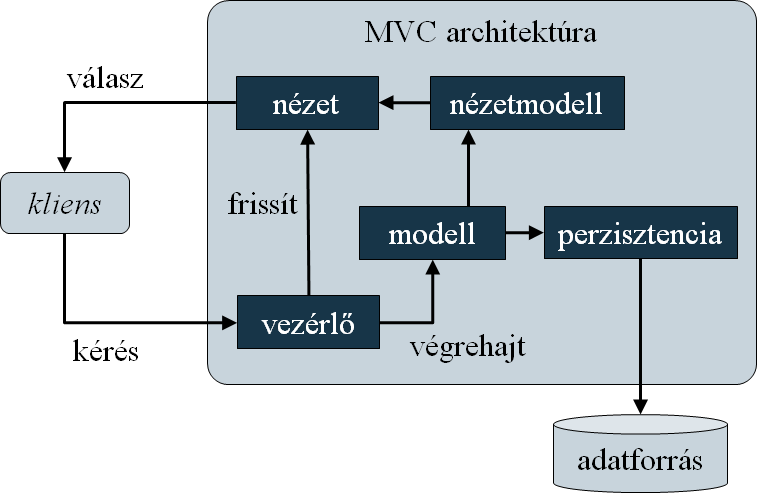
\includegraphics[width=1.0\textwidth]{developerguide/mvc-pattern}
	\caption{A Model-View-Controller architektúra}
	\label{fig:mvc-pattern}
\end{figure}
Az alkalmazásban a könnyebb és egyszerűbb fejleszthetőség miatt, a \emph{Model} réteget több komponensre bontjuk. Így az alábbi komponensekből áll össze a \emph{Model} réteg:
\begin{center}
	\begin{forest}
		for tree={
			font=\ttfamily,
			grow'=0,
			child anchor=west,
			parent anchor=south,
			anchor=west,
			calign=first,
			edge path={
			\noexpand\path [draw, \forestoption{edge}]
			(!u.south west) +(7.5pt,0) |- node[fill,inner sep=1.25pt] {} (.child anchor)\forestoption{edge label};
			},
			before typesetting nodes={
			if n=1
				{insert before={[,phantom]}}
				{}
			},
			fit=band,
			before computing xy={l=15pt},
		}
		[ASS
			[ASS.BLL/
				[Interfaces/]
				[Services/]
			]
			[ASS.DAL/
				[Models/]
				[ASSContext.cs]
				[DbInitializer.cs]
			]
			[ASS.WEB/
				[Models/
					[DTOs/]
					[ViewModels]
				]
			]
		]
	\end{forest}
\end{center}
\begin{description}
	\item[ASS.BLL:]  az üzleti logikai réteget megvalósító komponens (angolul \emph{Business Logic Layer}).
	\item[ASS.DAL:] az adatelérési réteget megvalósító komponens (angolul \emph{Data Access Layer}).
	\item[ASS.WEB.Models:] ebben a komponensben tároljuk az adatok bevitelére és az adatok megjelenítésére szolgáló osztályokat.
	\item[ASSContext.cs:] Az adatbázist leíró osztály.
	\item[DbInitializer.cs:] Az adatbázist létrehozó statikus osztály.    
\end{description}
\section{Logolás}
\label{sec:log}
Az alkalmazás fájl szintű logolást tartalmaz, amit a \emph{Serilog.Extensions.Logging.File} nyílt forráskódú programkönyvtár használatával valósítjuk meg \cite{SERILOG}. Az alkalmazás automatikusan logolja a futás közbeni eseményeket és az esetleges kivételeket. Természetesen támogatott a saját logüzenetek létrehozása is. A logolás beállításait az \emph{appsettings.json} (\ref{src:json} ábra) fájlban tudjuk személyreszabni. Az alábbi négy értéket szablyuk személyre az alkalmazáshoz:
\begin{itemize}
	\item PathFormat: itt tudjuk megadni az alkalmazás logfájljainak a mentési helyét, és egy sablont a fájlok nevére. A \emph{\{Date\}} paraméter helyére az aktuális dátum kerül beillesztésre (pl.: 20210513). Ha az elérési útban található mappa nem létezik azt a programkönyvtár automatikusan létrehozza a számunkra.
	\item OutputTemplate: itt adható meg a log üzenetek sablonja, hogy hogyan nézzenek ki a logolt üzenetek\footnote{Az \href{https://github.com/serilog/serilog/wiki/Formatting-Output}{alábbi linken} részletes leírást olvashatunk az \emph{OutputTemplate}-ben használható paraméterekről.}. Az alkalmazás a következő sablont használja a logokra: [\emph{Időbélyeg}] - [\emph{Log szintje}] - [\emph{Üzenet}] \emph{Új sor} [\emph{Kivétel (ha van)}].
	\item LogLevel: itt állíthatjuk be, hogy milyen minimum szintű események kerüljenek logolásra \cite{LogLevels}. A jelenlegi beállítással az alkalmazás minden legalább \emph{Information} szinttel rendelkező eseményt logol.
\end{itemize}
\newpage
\lstset{caption={Logolás beállításai}, label=src:json}
\begin{lstlisting}[language=json]
...
"Logging": {
	"PathFormat": "../Logs/log-{Date}.log",
	"OutputTemplate": "[{Timestamp:yyyy.MM.dd HH:mm:ss}] - [{Level:u}] - {Message}{NewLine}{Exception}",
	"LogLevel": {
		"Default": "Debug",
		"Microsoft": "Information"
	}
},
...
\end{lstlisting}
\section{Adatbázis}
\label{sec:database}
\subsection{Technológiák}
Az alkalmazáshoz szükséges telepítünk egy \emph{MySQL Community Server}-re, ajánlott a \emph{8.0.25}-ös verzió.\footnote{Az alkalmazás működik régebbi verzióval is. Viszont az alkalmazás nincs felkészítve az esetleges verziók közötti különbségekre.} Az autentikáció és autorizáció megvalósításához a Microsoft által készített \emph{Microsoft.AspNetCore.Identity.EntityFrameworkCore} nyílt forráskódú programkönyvtárat használja rendszer. A programkönyvtár tartalmaz meglévő adatbázis táblákat melyeknek a tartalma és működése elolvasható a Microsoft hivatalos honlapján \cite{Identity}. A programkönyvtár gondoskodik a jelszavak biztonságos tárolásáról, melyet időfüggő sózással és a jelszó hashelésével valósít meg.

Az adatbázis \emph{code first} módszerrel van megvalósítva, tehát nem az adatbázis szerveren \emph{SQL} kódot futattva hozzuk létre az adatbázis táblákat, hanem modell osztályokkal definiáljuk az adatbázis táblákat \cite{CodeFirst}. Ezen modelleket az \emph{ASS.DAL.Models} névtérben tároljuk.

Az adatelérést az \emph{Entity Framework Core ORM}\footnote{Jelentése: objektum-relációs leképzés, egy technika az adatok konvertálására nem kompatibilis típusos rendszerek és objektumorientált programozási nyelvek között.} keretrendszer biztosítja \cite{EFCore}. Így az alkalmazás forráskódjában nincsenek beégetett \emph{SQL} kódok. Ezek helyett a \emph{CRUD}\footnote{Create,Read,Update,Delete műveleteknek a rövidítése} műveleteket a \emph{.NET} nyújtotta és az \emph{Entity Framework Core} által is támogatott \emph{LINQ} (Language Integrated Queries) metódus hívásokkal valósul meg \cite{LINQ}. Továbbá a keretrendszer védelmet biztosít az \emph{SQL Injection} támadások ellen \cite{SQLInjection}, ugyanis a műveletek a \emph{C\#} és \emph{LINQ} metódusokból kerülnek előállításra paraméterezetten.

Az adatbázis elérését az alkalmazás konfigurációs fájljában (\emph{appsettings.json}) tudjuk megadni illetve módosítani.
\lstset{caption={Adatbázis elérése}, label=src:json}
\begin{lstlisting}[language=json]
...
"ConnectionStrings": {
	"DefaultConnection": "server=localhost;database=ASS;uid=username;password=fooBarraBoof"
},
...
\end{lstlisting}
\subsection{Az adatbázis táblái}
Az alkalmazás adatbázis diagramját a \ref{fig:dbdiagram} ábrán tekinthetjük meg. A \emph{Microsoft.AspNetCore.Identity.EntityFrameworkCore} keretrendszer által létrehozott táblákból csak azon a táblák és mezők kerülnek részletezésre, melyeket a rendszer aktívan használ. \footnote{A táblák amik nem kerülnek részletezésre a Microsoft hivatalos honlapján meg lehet tekinteni.}
\begin{figure}[H]
	\centering
	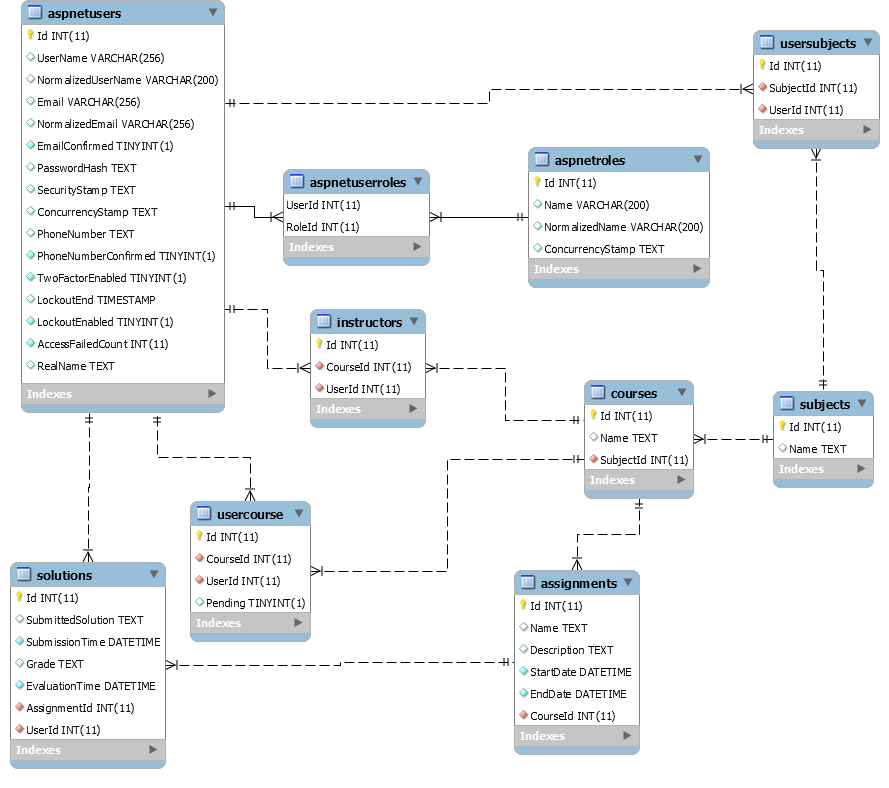
\includegraphics[width=1.0\textwidth]{developerguide/dbdiagram}
	\caption{Az adatbázis táblái}
	\label{fig:dbdiagram}
\end{figure}
\subsubsection{aspnetusers}
A \emph{Microsoft.AspNetCore.Identity.EntityFrameworkCore} programkönyvtár által automatikusan létrehozott tábla. A felhasználók adatait tárolja.
\begin{table}[H]
	\centering
	\begin{tabular}{ | m{0.25\textwidth} | m{0.25\textwidth} | m{0.40\textwidth} | }
		\hline
		\textbf{Mező neve} & \textbf{Típus} & \textbf{Leírás} \\
		\hline \hline
		Id & int & Elsődleges kulcs \\
		\hline
		UserName & string & Felhaszálónév (neptun kód) \\
		\hline
		Email & string & Felhasználó e-mail címe \\
		\hline
		RealName & string & Felhasználó neve \\
		\hline
		PasswordHash & string & Felhasználó hashelt jelszava \\
		\hline
	\end{tabular}
	\caption{Adatbázis: felhasználók táblája}
	\label{tab:db-users}
\end{table}
\section{Model réteg}
\label{sec:model}
\section{Vezérlő réteg}
\label{sec:controller}
\section{Nézet réteg}
\label{sec:view}